\chapter{Conclusions}
\label{chapter:conclusions}

This thesis has examined different technical solutions to managing, sharing and
publishing research data, focusing on sharing and publishing.
Table~\ref{table:solutions} shows the features of solutions presented and shows
how they differ in the context of research data publishing, whereas Table~\ref{table:management} shows the same solutions but in the context of research
data management during a research project. Table~\ref{table:legend_colors} shows the legend that is used in
Tables~\ref{table:solutions} and \ref{table:management}. Research data is referred
to as data in the tables for a more concise presentation. Later in this section the
proposed requirements for a successful research data management solution
are presented.

\captionof{table}{The color coding of the summary Tables \ref{table:solutions} and \ref{table:management}}
\addtocounter{table}{-1}
\label{table:legend_colors}
    \begin{tabularx}{\textwidth}{| >{\raggedright}p{3cm} | X |}
    \hline
    \textbf{Color and Mark} & \textbf{Meaning} \\
    \hline
    \multicolumn{1}{|c|}{\cellcolor{green}++} & The feature is well implemented and could be considered a strong point
                          in the solution \\
    \hline
    \multicolumn{1}{|c|}{\cellcolor{yellow}+} & The feature is implemented in the solutions in some way - it might need
                          some work to get up and running or the other features of the solution can be used to
                          approximate the functionality \\
    \hline
    \multicolumn{1}{|c|}{\cellcolor{red}-}    & The feature is missing from the solution or can be found from the solution but according
                          to user feedback is too hard to use and is a clear weak point of the solution \\
    \hline
\end{tabularx}

In Tables \ref{table:solutions} and \ref{table:management} the IDA, Etsin, Avaa and PAS are a part of the
Finnish Open Science Initiative. Dataverse, Hydra, Zenodo, iRODS and CKAN are
open source solutions. EUDAT refers to the B2-offering\footnote{\url{http://eudat.eu/}},
of which the B2Share and B2Drop are considered to be a part of a research
data management and publication process. ACRIS is the Elsevier Pure instance
that is being trialed at Aalto University. GitHub is included in the
comparison since it is a widely adopted tool for publishing and collaborating
on software projects.

The features used in the columns in Table \ref{table:solutions} are explained
in Table \ref{table:solution_features}.

\pagebreak

\captionof{table}{The features being compared on Table \ref{table:solutions}}
\addtocounter{table}{-1}
\label{table:solution_features}
    \begin{tabularx}{\textwidth}{| >{\raggedright}p{3cm} | X |}
    \hline
    \textbf{Feature} & \textbf{Explanation} \\
    \hline
    \rowcolor{Gray}
    Data Storage    & Data storage means that the solution offers the chance to
                      save the actual research data to the system and not just links
                      to the datasets, for example\\
    \hline
    Metadata Storage &  Metadata storage means that the system has a structured way
                        of storing metadata about datasets - this does not mean that
                        the system should contain actual research data, since some services
                        are built just as places to store metadata and links to datasets\\
    \hline
    \rowcolor{Gray}
    Open Access Data    & System that implements this feature allows the datasets to be searched
                          and downloaded by the general public without restrictions to the use
                          of the datasets\\
    \hline
    Restricted Data    & Whereas open access data is available for all the world to see, systems
                         that implement the restricted data feature allow for a more fine grained
                         user management allowing datasets to be shared with restricted groups
                         of users\\
    \hline
    \rowcolor{Gray}
    Long Term Archival    & Long term archival is archival for datasets that lasts for tens of years -
                            a lot longer than commodity hard drives last in active use (commodity
                            hard drives usually last from three to five years in active use)\\
    \hline
    Full Text Search    & Full text search refers to the ability to search the all the metadata
                          available in the system to find relevant datasets\\
    \hline
    \rowcolor{Gray}
    Dataset Versioning    & Dataset versioning means that the system allows for uploading newer versions
                           of the already uploaded datasets without deleting the old datasets, since
                           someone might use and refer to the old datasets\\
    \hline
    Identifier Scheme    & Identifier scheme tells which, if any, persistent identifier schemes the
                           solution implements\\
    \hline
\end{tabularx}

From the solutions presented in Table \ref{table:solutions} the systems that
are designed primarily for research data publishing (Avaa, Dataverse, Hydra,
Zenodo, and CKAN) have almost all the features specified. What some of
them are lacking is the ability to restrict access to the research data, which
is a requirement for some datasets that contain data that has some
confidentiality clauses. Avaa, for example, is a platform for nothing else than
completely open data making it an awkward choice for a university, for example.
None of these solutions implement long term archival,
which is an important feature going forward and a goal for future development.
These solutions are also remarkably similar, so any one of them could be used
to set up a research data publishing platform for a research institution.

The only solution for long term archival is PAS, which is in test phase as of
writing of this thesis. It ticks many boxes of the features, but it has to be
taken into account that the PAS system is only for long term archival and
can not be used for the normal publishing activity of research institutions.
It is also unclear at the moment how datasets for long term archival are
chosen, what kind of metadata long term archival requires and how the system
should integrate to existing and upcoming research data repositories.

The tools that have a lot of other functionality in addition to research data
publishing implement the features to a varying degree. iRODS, which is a tool
for managing data, is clearly not designed to be a data sharing platform for
research data. ACRIS has many other tasks as well, such as maintaining a the
publication profile of researchers and reporting publications. EUDAT's B2Share
offering offers a serviceable research data publication platform, but lacks the
ability to restrict access to the datasets in a fine grained manner. IDA is an iRODS based system, but
has some features for publishing datasets from the system. Biggest problem with
it is that it is perceived very hard to use by users.

Etsin is a metadata publication platform - it only contains metadata and links
to the actual location of the datasets. While this is valuable, separating the
research data from the metadata requires either integration between the storage
and metadata systems or more work from the users. This is also the reason why
Open Access Data is marked as a weakness of the system - no data, no open access.

The identifier scheme is also a point of interest. Citing datasets is something
that has not been widely adopted, which means that in order to help that
adoption a well known identifier scheme should be used. It is good that
a Finnish identifier scheme exists, but if datasets want international recognition
an internationally known identifier scheme should be used.

The technical solutions with a focus on research data publishing fill their
role adequately. The user tests show that there are user experience and
usability improvements that could be done - those are detailed in Section
\ref{sec:prototype_outcomes}. What the user tests also show is that training
related to the options when it comes to research data publishing is lacking.
If the culture and willingness to share research data is to be improved,
that would require a conscious effort from the university side.

\begin{sidewaystable}[h]
    \caption{Existing solutions in light of research data publishing}
    \label{table:solutions}
    \resizebox{\textwidth}{!}{
        \renewcommand{\arraystretch}{2.0}
        \begin{tabular}{| l | c | c | c | c | c | c | c | c | c |}
            \cline{3-10}\cline{1-1}
            \rowcolor{top-level-blue}
            \vspace{1 mm}
            \textbf{Tool} &\cellcolor{white}& \textbf{Data Storage} & \textbf{Metadata Storage} & \textbf{Open Access Data} & \textbf{Restricted Data} & \textbf{Long Term Archival} & \textbf{Full Text Search} & \textbf{Dataset Versioning} & \textbf{Identifier Scheme} \\
            \cline{3-10}\cline{1-1}
            \cellcolor{first-column-blue}IDA     && \cellcolor{green}++ & \cellcolor{yellow}+ & \cellcolor{yellow}+  & \cellcolor{yellow}+  & \cellcolor{red}-  &  \cellcolor{green}++ & \cellcolor{red}-  & \cellcolor{green}URN \\
            \cline{3-10}\cline{1-1}
            \cellcolor{first-column-blue}Etsin   && \cellcolor{red}-  & \cellcolor{green}++ & \cellcolor{red}-  & \cellcolor{red}-  & \cellcolor{red}-  &  \cellcolor{green}++ & \cellcolor{red}-  & \cellcolor{green}URN \\
            \cline{3-10}\cline{1-1}
            \cellcolor{first-column-blue}Avaa    && \cellcolor{green}++ & \cellcolor{green}++ & \cellcolor{green}++ & \cellcolor{red}-  & \cellcolor{red}-  &  \cellcolor{green}++ & \cellcolor{red}-  & \cellcolor{green}URN \\
            \cline{3-10}\cline{1-1}
            \cellcolor{first-column-blue}Dataverse && \cellcolor{green}++ & \cellcolor{green}++ & \cellcolor{green}++  & \cellcolor{green}++ & \cellcolor{red}-  &  \cellcolor{green}++ & \cellcolor{yellow}+  & \cellcolor{green}DOI/Handle \\
            \cline{3-10}\cline{1-1}
            \cellcolor{first-column-blue}Hydra    && \cellcolor{green}++ & \cellcolor{green}++ & \cellcolor{green}++ & \cellcolor{green}++ & \cellcolor{red}-  &  \cellcolor{green}++ & \cellcolor{yellow}+  & \cellcolor{green}DOI \\
            \cline{3-10}\cline{1-1}
            \cellcolor{first-column-blue}Zenodo   && \cellcolor{green}++ & \cellcolor{green}++ & \cellcolor{green}++ & \cellcolor{yellow}+  & \cellcolor{red}-  &  \cellcolor{green}++ & \cellcolor{yellow}+  & \cellcolor{green}DOI \\
            \cline{3-10}\cline{1-1}
            \cellcolor{first-column-blue}EUDAT    && \cellcolor{green}++ & \cellcolor{green}++ & \cellcolor{green}++ & \cellcolor{yellow}+  & \cellcolor{red}-  &  \cellcolor{green}++ & \cellcolor{yellow}+  & \cellcolor{green}Handle \\
            \cline{3-10}\cline{1-1}
            \cellcolor{first-column-blue}iRODS    && \cellcolor{green}++ & \cellcolor{yellow}+ & \cellcolor{red}-  & \cellcolor{red}-  & \cellcolor{red}-  &  \cellcolor{green}++ & \cellcolor{yellow}+  & \cellcolor{red}- \\
            \cline{3-10}\cline{1-1}
            \cellcolor{first-column-blue}CKAN     && \cellcolor{green}++ & \cellcolor{green}++ & \cellcolor{green}++ & \cellcolor{green}++ & \cellcolor{red}-  &  \cellcolor{green}++ & \cellcolor{yellow}+  & \cellcolor{yellow}+ \\
            \cline{3-10}\cline{1-1}
            \cellcolor{first-column-blue}ACRIS    && \cellcolor{red}-  & \cellcolor{yellow}+  & \cellcolor{yellow}+  & \cellcolor{yellow}+  & \cellcolor{red}-  &  \cellcolor{green}++ & \cellcolor{red}-  & \cellcolor{yellow}+ \\
            \cline{3-10}\cline{1-1}
            \cellcolor{first-column-blue}PAS      && \cellcolor{green}++ & \cellcolor{green}++ & \cellcolor{green}++ & \cellcolor{red}-  & \cellcolor{green}++ &  \cellcolor{green}++ & \cellcolor{red}-  & \cellcolor{green}URN \\
            \cline{3-10}\cline{1-1}
            \cellcolor{first-column-blue}GitHub   && \cellcolor{green}++ & \cellcolor{yellow}+  & \cellcolor{green}++ & \cellcolor{green}++ & \cellcolor{red}-  &  \cellcolor{green}++ & \cellcolor{green}++ & \cellcolor{green}DOI \\
            \cline{3-10}\cline{1-1}
        \end{tabular}
    }
\end{sidewaystable}

\clearpage

\iffalse
\begin{sidewaysfigure}
    \begin{centering}
        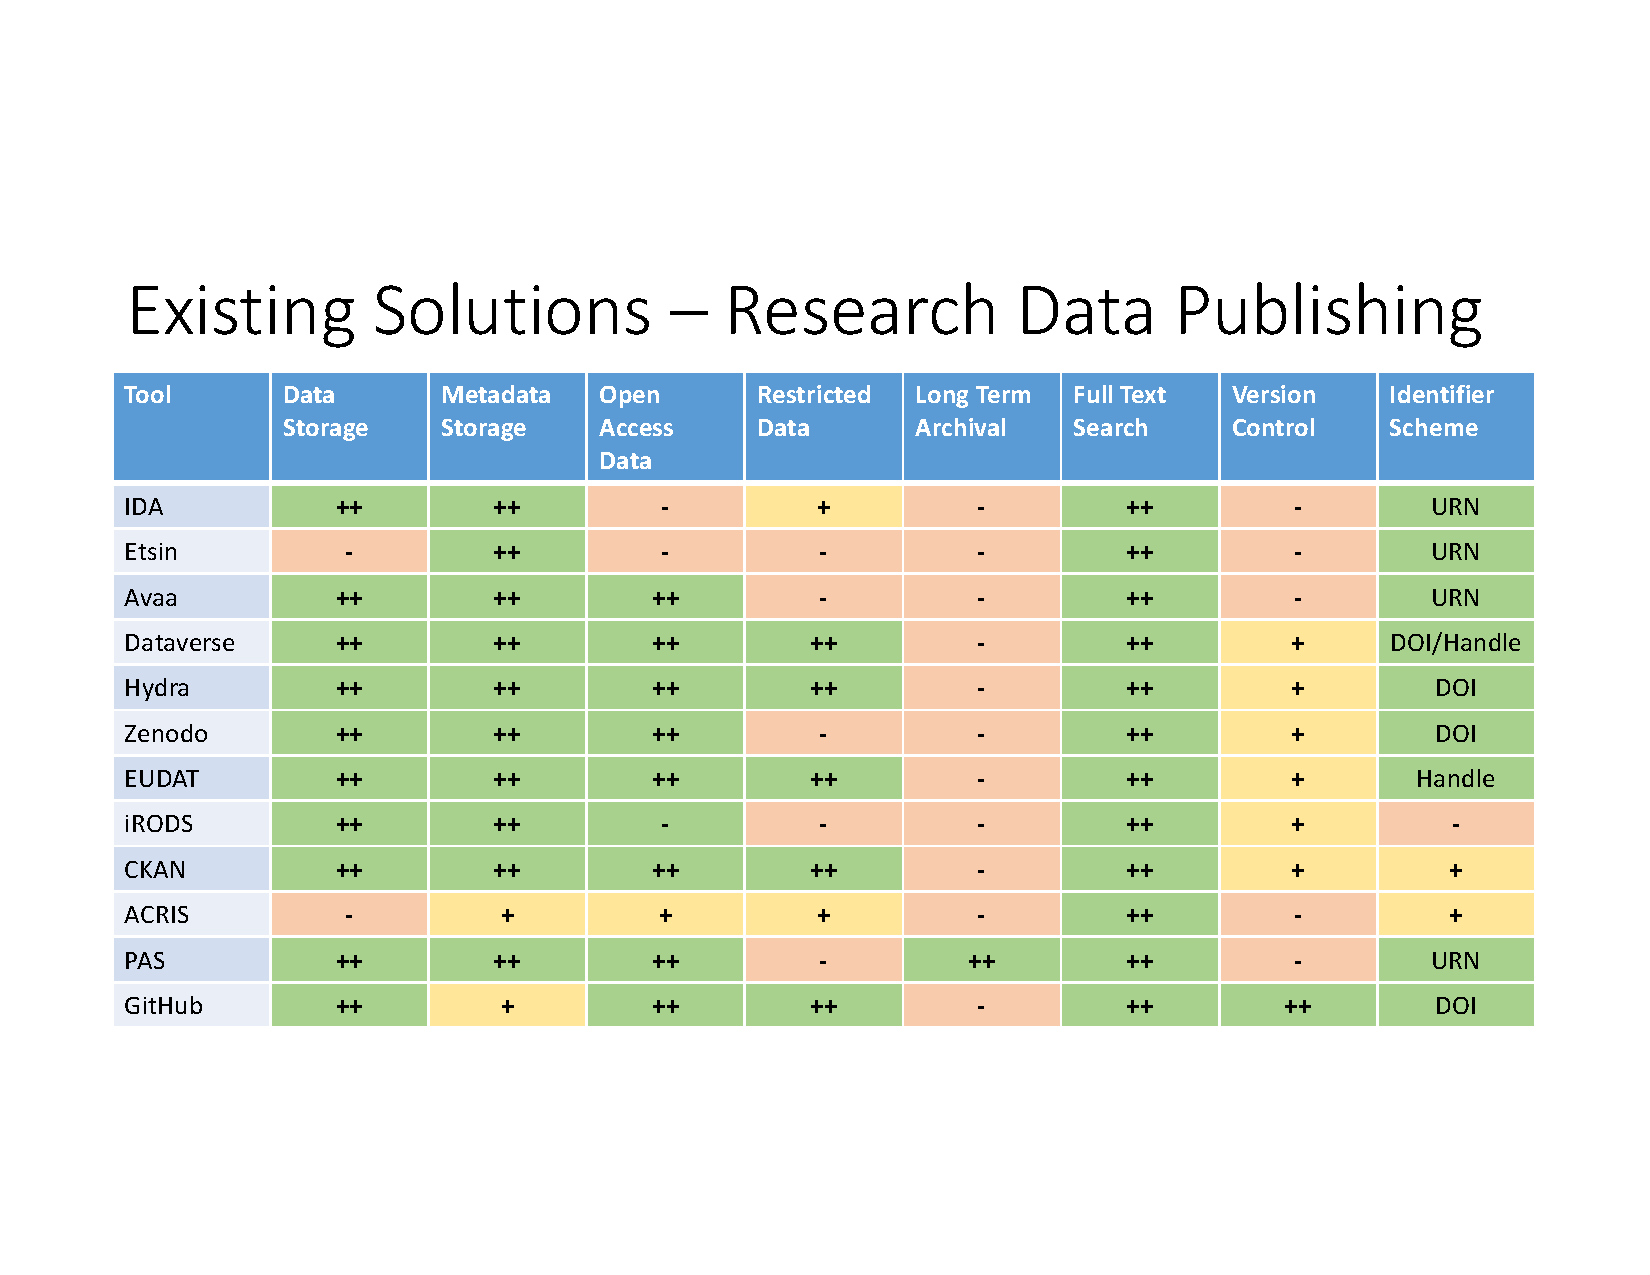
\includegraphics[width=\textwidth]{images/publishing}
    \end{centering}
    \caption{A placeholder for the latex table}
    \label{fig:solutions}
\end{sidewaysfigure}
\fi

Research data publishing is the end goal of research data management, and
Table \ref{table:management} shows the same tools compared previously in
the context of research data publishing being compared in the light
of research data management during the research process. Table
\ref{table:management_features} explains the features that were
explored from the research data management angle.

\captionof{table}{The features being compared on Table \ref{table:management}}
\addtocounter{table}{-1}
\label{table:management_features}
    \begin{tabularx}{\textwidth}{| >{\raggedright}p{3cm} | X |}
    \hline
    \textbf{Feature} & \textbf{Explanation} \\
    \hline
    \rowcolor{Gray}
    File Sharing With Partners    & The basis of collaboration is sharing results and in this
                                    context it means that the solution enables files to be
                                    shared using the system - this also implies that the files
                                    can be stored there for personal use\\
    \hline
    File Editing With Partners & For collaboration just sharing files might not be enough, and
                                 the files should be able to be edited instead of always uploading
                                 new versions to the system\\
    \hline
    \rowcolor{Gray}
    Workflow Sharing    &  The research workflows in some fields of science are highly automated
                           and sharing those would save a lot of time for collaborators and the person
                           sharing them assuming he or she had to return to that workflow later\\
    \hline
    Comments On Files    & Commenting on others' work makes collaboration easier\\
    \hline
    \rowcolor{Gray}
    Web Interface          & A system implements this feature if it has an interface online that
                             can be accessed from anywhere so that the research data is readily
                             accessible\\
    \hline
    Command Line Interface    & A system implements a command line interface if the users can access
                                their research data using technologies like SSH\\
    \hline
    \rowcolor{Gray}
    Desktop Interface       & A system implements a desktop interface if it offers software that the
                              users can install on their personal machines or it integrates to the
                              file system on the user's machine\\
    \hline
    Integrated Data Collection    & Integrated data collection means that tools that collect research
                                    data can be integrated to the solution such that the research data
                                    is collected and put into the systems automatically\\
    \hline
\end{tabularx}

The same tools that are suitable for research data publishing are not
necessarily right for research data management and vice versa. iRODS, IDA
and the B2Drop side of the EUDAT service offer dedicated services to share research data during
the research process and manage it in a centralized service. GitHub is a
collaborative tool for projects around programming.

The tools that work well for research data publishing lack many important
features that research data management and research collaboration, such
as file editing and proper commenting functionality on file. Research workflows
cannot be stored or shared with any of the tools, which is not surprising - the
definition of a workflow varies a lot between disciplines and it is not a
requirement for many.

The user tests and interviews also show that the research management ways
of researchers could be much better. Research data management is learned
by doing and from peers and the awareness of good practices and tools for
research data management is low. Good practices and tools should be taught to
the researchers creating and managing the research data.

\begin{sidewaystable}
    \caption{Existing solutions in light of research data management}
    \label{table:management}
    \resizebox{\textwidth}{!}{
        \renewcommand{\arraystretch}{2.0}
        \begin{tabular}{| l | c |c | c | c | c | c | c | c | c |}
            \cline{3-10}\cline{1-1}
            \rowcolor{top-level-blue}
            \vspace{1 mm}
            \textbf{Tool} &\cellcolor{white}& \textbf{\vtop{\hbox{\strut File Sharing}\hbox{\strut With Partners}}} & \textbf{\vtop{\hbox{\strut File Editing}\hbox{\strut  With Partners}}} & \textbf{Workflow Sharing} & \textbf{Comments On Files} & \textbf{Web Interface} & \textbf{\vtop{\hbox{\strut Command Line}\hbox{\strut Interface}}} & \textbf{Desktop Interface} & \textbf{\vtop{\hbox{\strut Integrated}\hbox{\strut Data Collection}}} \\
            \cline{3-10}\cline{1-1}
            \cellcolor{first-column-blue}IDA         && \cellcolor{green}++ & \cellcolor{green}++ & \cellcolor{red}-  & \cellcolor{yellow}+  & \cellcolor{green}++  &  \cellcolor{green}++ & \cellcolor{green}++  & \cellcolor{yellow}+ \\
            \cline{3-10}\cline{1-1}
            \cellcolor{first-column-blue}Etsin       && \cellcolor{red}-  & \cellcolor{red}- & \cellcolor{red}-  & \cellcolor{red}-  & \cellcolor{green}++  &  \cellcolor{green}++ & \cellcolor{red}-  & \cellcolor{red}- \\
            \cline{3-10}\cline{1-1}
            \cellcolor{first-column-blue}Avaa        && \cellcolor{green}++ & \cellcolor{red}- & \cellcolor{red}- & \cellcolor{red}-  & \cellcolor{green}++  &  \cellcolor{green}++ & \cellcolor{red}-  & \cellcolor{red}- \\
            \cline{3-10}\cline{1-1}
            \cellcolor{first-column-blue}Dataverse   && \cellcolor{green}++ & \cellcolor{red}- & \cellcolor{red}-  & \cellcolor{yellow}+ & \cellcolor{green}++  &  \cellcolor{green}++ & \cellcolor{red}-  & \cellcolor{red}- \\
            \cline{3-10}\cline{1-1}
            \cellcolor{first-column-blue}Hydra       && \cellcolor{green}++ & \cellcolor{red}- & \cellcolor{red}- & \cellcolor{yellow}+ & \cellcolor{green}++  &  \cellcolor{green}++ & \cellcolor{red}-  & \cellcolor{red}- \\
            \cline{3-10}\cline{1-1}
            \cellcolor{first-column-blue}Zenodo      && \cellcolor{green}++ & \cellcolor{red}- & \cellcolor{red}- & \cellcolor{yellow}+  & \cellcolor{green}++  &  \cellcolor{green}++ & \cellcolor{red}-  & \cellcolor{red}- \\
            \cline{3-10}\cline{1-1}
            \cellcolor{first-column-blue}EUDAT       && \cellcolor{green}++ & \cellcolor{green}++ & \cellcolor{red}- & \cellcolor{yellow}+  & \cellcolor{green}++  &  \cellcolor{green}++ & \cellcolor{green}++  & \cellcolor{red}- \\
            \cline{3-10}\cline{1-1}
            \cellcolor{first-column-blue}iRODS       && \cellcolor{green}++ & \cellcolor{green}++ & \cellcolor{red}-  & \cellcolor{yellow}+  & \cellcolor{green}++  &  \cellcolor{green}++ & \cellcolor{green}++  & \cellcolor{green}++ \\
            \cline{3-10}\cline{1-1}
            \cellcolor{first-column-blue}CKAN        && \cellcolor{green}++ & \cellcolor{red}- & \cellcolor{red}- & \cellcolor{yellow}+ & \cellcolor{green}++  &  \cellcolor{green}++ & \cellcolor{red}-  & \cellcolor{red}- \\
            \cline{3-10}\cline{1-1}
            \cellcolor{first-column-blue}ACRIS       && \cellcolor{green}++  & \cellcolor{red}-  & \cellcolor{red}-  & \cellcolor{red}-  & \cellcolor{green}++  &  \cellcolor{green}++ & \cellcolor{red}-  & \cellcolor{red}- \\
            \cline{3-10}\cline{1-1}
            \cellcolor{first-column-blue}PAS         && \cellcolor{green}++ & \cellcolor{red}- & \cellcolor{red}- & \cellcolor{red}-  & \cellcolor{green}++ &  \cellcolor{green}++ & \cellcolor{red}-  & \cellcolor{red}- \\
            \cline{3-10}\cline{1-1}
            \cellcolor{first-column-blue}GitHub      && \cellcolor{green}++ & \cellcolor{green}++  & \cellcolor{red}- & \cellcolor{green}++ & \cellcolor{green}++  &  \cellcolor{green}++ & \cellcolor{green}++ & \cellcolor{red}- \\
            \cline{3-10}\cline{1-1}
        \end{tabular}
    }
\end{sidewaystable}

\iffalse
\begin{sidewaysfigure}
    \begin{centering}
        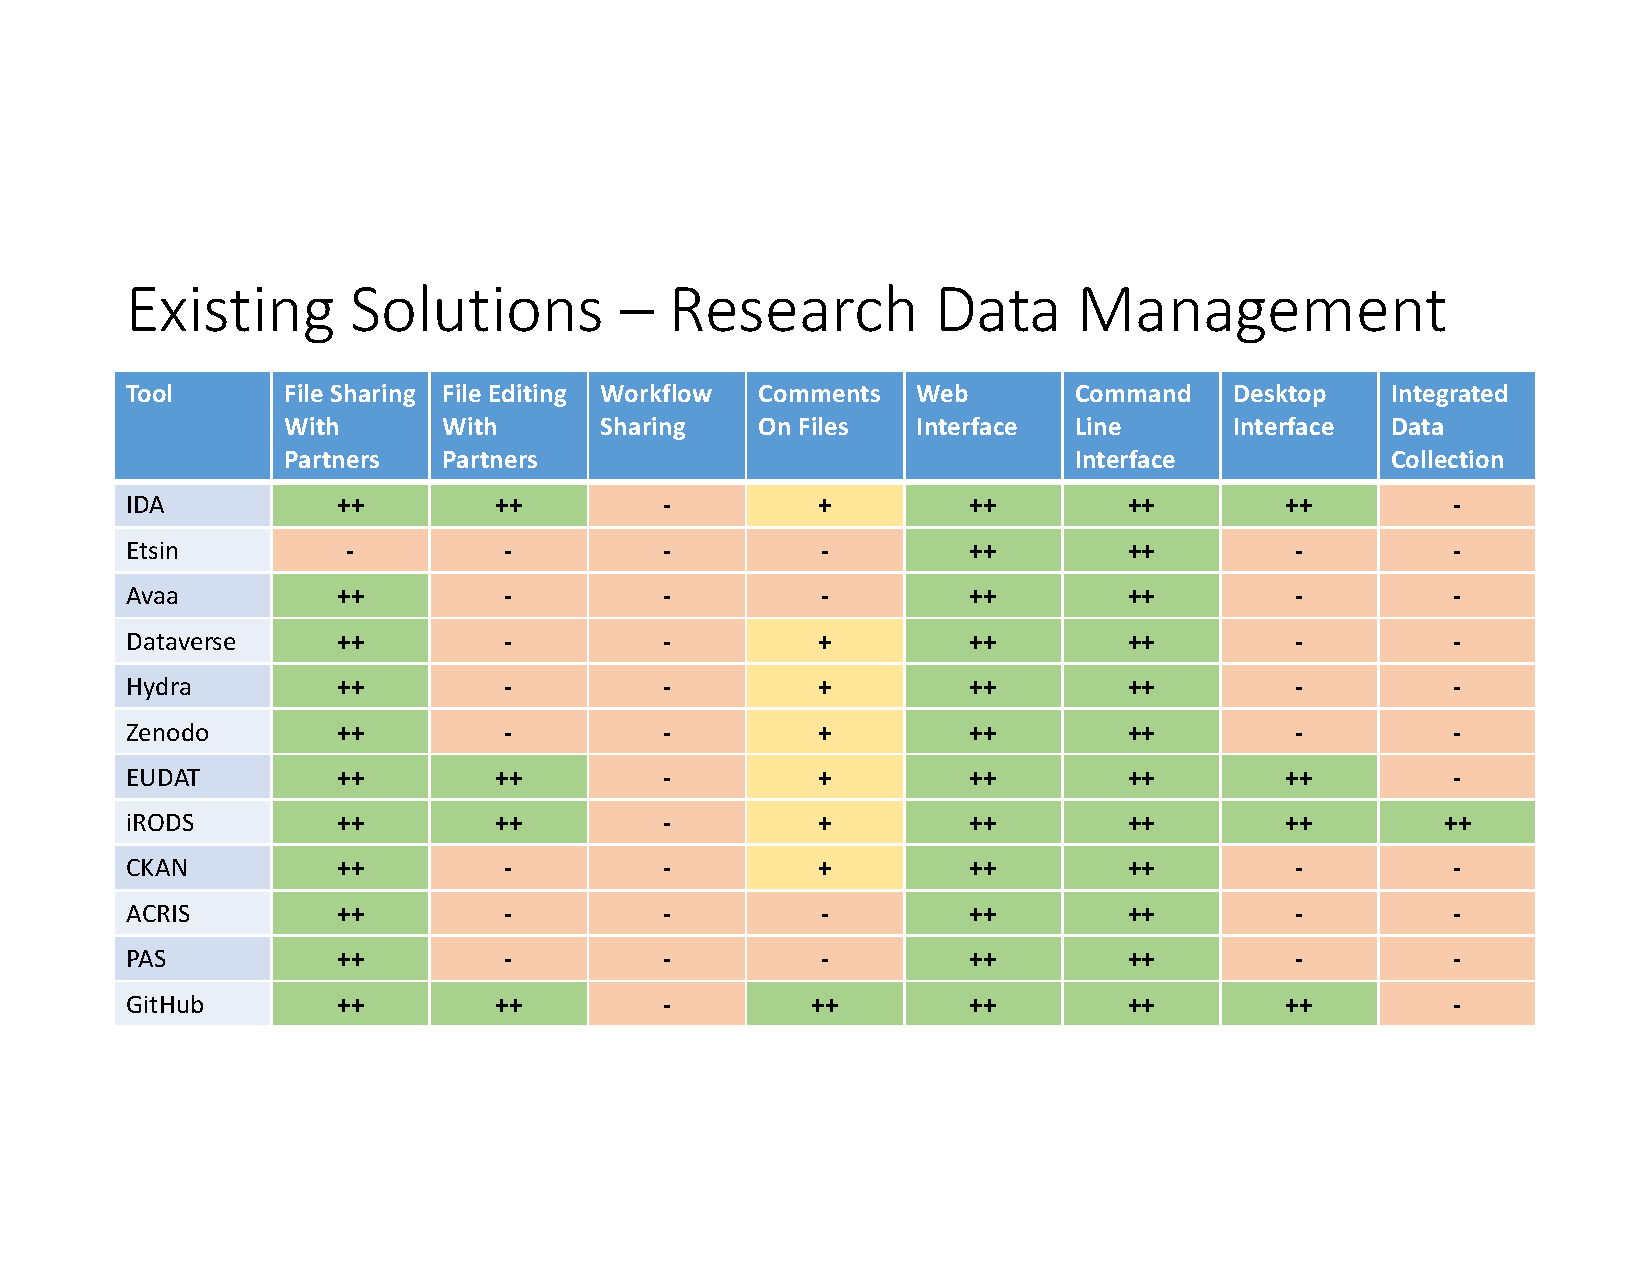
\includegraphics[width=\textwidth]{images/management}
    \end{centering}
    \caption{A placeholder for the latex table}
    \label{fig:management}
\end{sidewaysfigure}
\fi


When looking at the existing solutions through both the context of research
data management and publishing it is clear that a big problem is that there
is not a solution that would handle the entire lifecycle of the data from
creation to publishing. Research data sharing and managing should not be considered
separately from research data management. Without management, there can not be
effective sharing or publishing and without sharing or publishing there is no
need for management. Many universities, Aalto University included, have
implemented neither managing or publishing research data tools in a centralized
way. The lack of dedicated research data management
infrastructure also affects the training and knowledge of research data
management and tools in the sense that if there is no infrastructure to
leverage there is no way to teach institutional best practices.

\clearpage

This thesis has also identified many aspects of a solution that could solve the
research data management and sharing problems. These requirements are split into
must have requirements, functional requirements, hardware requirements and
user experience requirements. Other than the must have requirements that a
system either does or does not fulfill the requirements contain metrics that
can be used to validate if the system fulfills the requirement. The
requirements presented here are formed to be quite general,
which means that in order to use them to design a solution the metrics
presented in the requirements should be made more specific. The requirements
are also not instructions set in stone - they should be used to guide in
developing a research data management and publishing system.

The must have -requirements are presented in Tables \ref{table:must_have_publishing} and
\ref{table:must_have_management}. The other requirements are presented in Appendix
\ref{chapter:reqs}.

\captionof{table}{Must have requirements for a research data publishing solution}
\addtocounter{table}{-1}
\label{table:must_have_publishing}
    \begin{tabularx}{\textwidth}{| >{\raggedright}p{3cm} | X |}
    \hline
    \textbf{Requirement} & \textbf{Rationale} \\
    \hline
    \rowcolor{Gray}
    Users can upload datasets    & Without datasets, there is not research data publishing\\
    \hline
    User can upload relevant metadata for their datasets & Without metadata, finding and reusing research data is impossible\\
    \hline
    \rowcolor{Gray}
    The metadata of datasets is full text searchable    &  In order to find datasets, the metadata has to be searchable\\
    \hline
    Published datasets are assigned a persistent identifiers    & Persistent identifiers allow for referencing the data and maintaining links for longer\\
    \hline
    \rowcolor{Gray}
    There are no restrictions to the type of uploaded data          & Research data comes in many shapes and forms and all data must be able to be published\\
    \hline
    The datasets in the system can be made public for all the world to see    & The goal of the publishing platform is to make the data public\\
    \hline
\end{tabularx}

\pagebreak

\captionof{table}{The must have requirements of a research data management solution}
\addtocounter{table}{-1}
\label{table:must_have_management}
    \begin{tabularx}{\textwidth}{| >{\raggedright}p{3cm} | X |}
    \hline
    \textbf{Requirement} & \textbf{Rationale} \\
    \hline
    \rowcolor{Gray}
    Users can upload their research data during the research project    & Instead of per researcher storage solution for storing research data, there must be a centralized solution\\
    \hline
    The tool imposes no restrictions to the type of research data stored & Research data comes in all shapes and forms and the tool must serve all the disciplines\\
    \hline
    \rowcolor{Gray}
    The research data management tool must allow for sharing data with collaborators    &  Research is done globally and collaboratively nowadays, meaning that data must be shared with collaborators\\
    \hline
\end{tabularx}
